\documentclass[11pt,DIV=12,parskip=half,headings=normal,abstract]{scrartcl}

\usepackage[T3,T1]{fontenc}
\usepackage[utf8]{inputenc}
\usepackage[ngerman]{babel}
\usepackage{amsmath}
\usepackage{amsfonts}
\usepackage[standard]{ntheorem}
\usepackage{amscd}
\usepackage{mathtools}
\usepackage{stmaryrd}
\usepackage{faktor}
\usepackage{enumerate}
\usepackage{wrapfig}
\usepackage[safe]{tipa} % for \textlambda

\usepackage[pdfauthor={Joachim Breitner},pdftitle={Haskell Bytes},pdfsubject={Eine Führung durch den Hauptspeicher eines Haskell-Programms}]{hyperref}
\usepackage{listings}
\usepackage{multicol}
\usepackage{ragged2e}
%\usepackage[para]{footmisc}
\usepackage{fourier}
\usepackage{microtype}
\usepackage{comment}

\usepackage{tikz}
\usetikzlibrary{shapes.geometric}
\usetikzlibrary{calc}
\usetikzlibrary{shapes.multipart}
\usetikzlibrary{arrows}

\urlstyle{sf}

\author{Joachim Breitner\footnote{\href{mailto:mail@joachim-breitner.de}{mail@joachim-breitner.de}, \url{http://www.joachim-breitner.de/}. Diese Arbeit wurde durch ein Promotionsstipendium der \href{http://telekom-stiftung.de/}{Deutschen Telekom Stiftung} gefördert.}}
\title{Haskell Bytes}
%\subject{Die Umsetzung von Haskell durch GHC}
\subtitle{Eine geführte Tour durch den Hauptspeicher eines Haskell-Programms}
\publishers{MRMCD 12\footnote{\url{http://mrmcd.net/}}, Darmstadt}
\date{8. September 2012}


\definecolor{light-gray}{gray}{0.95}
\lstdefinestyle{basic}{
        ,columns=flexible
        ,basewidth={.365em}
        ,keepspaces=True
	,belowskip=0pt
	,backgroundcolor=\color{light-gray}
	,frame=single
	,xleftmargin=2em
	,xrightmargin=2em
        ,basicstyle=\small\sffamily
        ,stringstyle=\itshape
}
\lstdefinestyle{haskell}{
	style=basic
	,language=Haskell
	,literate=
		{ö}{{\"o}}1
	        {ä}{{\"a}}1
                {ü}{{\"u}}1
        ,texcl=true
        ,showstringspaces=false
        ,keywords={module,where,open,import,using,renaming,to,data,let,in,with}
}

\newcommand{\mylabel}[1]{\raisebox{2em}[0pt][0pt]{\makebox[0pt][l]{\makebox[\linewidth][r]{\color{gray}{\sffamily #1}\hspace{2em}}}}\ignorespaces}
\lstnewenvironment{haskell}{\lstset{style=haskell}}{\mylabel{Haskell}\pagebreak[2]}
\lstnewenvironment{ghci}{\lstset{style=haskell}}{\mylabel{GHCi}\pagebreak[2]}
\lstnewenvironment{shell}{\lstset{style=basic}}{\mylabel{Shell}}
\newcommand{\inputhaskell}[1]{\lstinputlisting[style=haskell]{#1}\mylabel{Haskell}}
\newcommand{\li}{\lstinline[style=haskell]}


\begin{document}

\maketitle

Haskell ist eine tolle Programmiersprache; ich schätze ihr das alle schon wisst, sonst wärt ihr wohl nicht in meinem Vortrag. Aber manchmal wird man von Haskella auch enttäuscht. Nehmen wir folgenden Code:
\begin{haskell}
main = do
    input <- getContents
    putStrLn $ "I read " ++ show (length input) ++ " bytes."
    putStrLn $ "The last line is:"
    putStrLn $ last (lines input)
\end{haskell}
und füttern ihn mit einer 100MB großen Textdatei. Mit dem Parameter \texttt{-RTS -t} können wir uns Statistiken anzeigen lassen und erfahren, dass das Programm 2521MB Speicher braucht – über 24$\times$ zu viel!

Ein anderes, klassiches Beispiel für unerwartetes Laufzeitverhalten ist der folgende Code, der die länge einer Liste zählt:
\lstinputlisting[style=haskell,linerange=3-6]{Count.hs}\mylabel{Haskell}
Im Interpreter sehen wir, dass der Code unnötig viel Speicher verbraucht und dann mit einem Stack Overflow abbricht:
\begin{ghci}
*Count> let x = count 0 [0..100000000]
*Count> x
Just *** Exception: stack overflow
\end{ghci}

Manchmal aber überrascht uns Haskell auch positiv. Wenn wir, wieder beim ersten Programm, die dritte Zeile löschen und
\begin{haskell}
main = do
    input <- getContents
    putStrLn $ "The last line is:"
    putStrLn $ last (lines input)
\end{haskell}
laufen lassen haben wir plötzlich einen Speicherverbrauch von 2MB – das ist 50$\times$ besser als erwartet! Und dann gibt es ja auch noch die unendlichen Listen in Haskell\dots

\section{Die Akteure}

Fragen wir uns also, was ein Haskell-Programm während der Ausführung alles im Speicher vorhalten muss. Zuerst wären da natürlich die eigentlichen \emph{Daten}, also Konstruktoren wie \li-True- oder \li-Just- oder \li-(,)-, die wiederum andere Werte enthalten können. Weiter ist Haskell ja eine funktionale Sprache die sich dadurch auszeichnet, dass man Funktionen selbst wie Daten behandeln kann. Also müssen wir auch \emph{Funktionen} speichern können. Und zuletzt ist Haskell lazy, das heißt es gibt Werte die noch nicht ausgewertet sind. Diese heißen \emph{Thunks}. Das sind schon mal die wichtigsten; allgemein spricht man hierbei von \emph{Closures}.

Bevor wir nun in den Speicher eines Haskell-Programms reinschauen überlegen wir noch, was denn jeweils zu so einer Funktion gespeichert werden soll.
\begin{itemize}
\item Der Typ eines Wertes: Der ist tatsächlich nicht nötig! Das Typsystem stellt sicher dass jeglicher Code stets Werte von Typ vorfindet, den er erwartet, er kann also blind drauf vertrauen. Das ist ganz anders als z.B. in Python!
\item Welcher Konstruktor: Ja, das muss man speichern, zumindest für Typen mit mehreren, etwa bei \li-data Maybe a = Just a | Nothing-.
\item Die Parameter des Konstruktors: Natürlich!
\item Bei Funktionen: Der Code der Funktion.
\item Nicht vergessen bei Funktionen und Thunks: Freie Variablen!
\end{itemize}

\subsection{Konstruktoren}

Schauen wir mal an was wir vorfinden, wenn wir mit GHCi etwas rumspielen, und fangen mit einer einfachen Zahl an:
\begin{ghci}
*Utils> let eins = 1 :: Int
*Utils> viewClosure eins
0x00007f9c7a3337f8: 0x0000000040502608 0x0000000000000001
\end{ghci}

Wir sehen also dass wir für einen Integer-Wert zwei Worte, die auf meiner Maschine jeweils 8 Bytes groß sind, benötigen. Das zweite speichert offensichtlich die eigentliche Zahl.

Wie sieht es mit Zeichen, also Charakters aus?
\begin{ghci}
*Utils> let zett = 'z'
*Utils> viewClosure zett
0x00007f9c7a0e8238: 0x0000000040502548 0x000000000000007A
\end{ghci}
Auch diese benötigen zwei Wörter, also 16 statt einem Byte! 

Kommen wir nun zu algebraischen Datentypen, und packen \li-eins- in \li-Just-:
\begin{ghci}
*Utils> let jeins = Just eins
*Utils> viewClosure jeins
0x00007f9c7b082710: 0x00000000420DC920 0x00007f9c7a3337f8
\end{ghci}

Beachte dass im Wert \li-Just eins- keine Kopie von \li-eins- gespeichert ist, sondern eine Referenz drauf.
%Das ist aus zwei Gründen wichtig: \li-eins- könnte sehr groß sein, dann will man es natürlich nicht kopieren. Und es gibt Funktionen die mit \li-Maybe a- für beliebige Typen \li-a- arbeiten. Die wissen nicht dass \li-Just eins- ein Integer enthält. Würde man jetzt den Wert direkt reinkopieren wäre 

Nun wollen wir verstehen, warum unser erstes Beispielprogramm so viel Speicher brauchte. Dazu erinnern wir uns dass der Typ \li-String- in Haskell nur eine Alias für \li-[Char]-, also Listen von Zeichen, ist.
\begin{ghci}
*Utils> let hallo = "hallo"
*Utils> viewListClosures hallo
0x00007f9c7ba21fa0: 0x0000000040502668 0x00007F9C7BA21F91 0x00007F9C7BA21F70
0x00007f9c7ba21f90/1: 0x0000000040502548 0x0000000000000068
0x00007f9c7ba77b18: 0x0000000040502668 0x00007F9C7BA77B09 0x00007F9C7BA77AE8
0x00007f9c7a1a9768/1: 0x0000000040502548 0x0000000000000061
0x00007f9c7ba405f0: 0x0000000040502668 0x00007F9C7BA405E1 0x00007F9C7BA405C0
0x00007f9c7ba405e0/1: 0x0000000040502548 0x000000000000006C
0x00007f9c7ba83f38: 0x0000000040502668 0x00007F9C7BA83F29 0x00007F9C7BA83F08
0x00007f9c7ba83f28/1: 0x0000000040502548 0x000000000000006C
0x00007f9c7ba55a20: 0x0000000040502668 0x00007F9C7BA55A11 0x00007F9C7BA559F0
0x00007f9c7a01e840/1: 0x0000000040502548 0x000000000000006F
0x0000000040507e70: 0x0000000040502648
\end{ghci}
Wir sehen nun dass die Liste \li-"hallo"- erst einmal aus einem Closure mit drei Wörtern besteht. Das zweite ist ein Pointer auf ein Closure für \li-'h'- und das dritte ein Pointer auf \li-"allo"-, und so weiter, bis wir bei der leeren Liste \li-[]- angekommen sind. Man beachte die deutlich andere Adresse: \li-[]- gibt es global nur einmal und lebt im statischen Codebereich.

An der Stelle will ich demonstrieren warum man in GHC keinen Zugriff auf die eigentlichen Pointer haben sollte:
\begin{ghci}
*Utils> System.Mem.performGC
*Utils> viewListClosures hallo
0x00007f9c7a1510a8: 0x0000000040502668 0x00007F9C7A151389 0x00007F9C7A151372
0x00007f9c7a151388/1: 0x0000000040502548 0x0000000000000068
0x00007f9c7a151370: 0x0000000040502668 0x00007F9C7A1516F1 0x00007F9C7A1516DA
0x00007f9c7a1516f0/1: 0x0000000040502548 0x0000000000000061
0x00007f9c7a1516d8: 0x0000000040502668 0x00007F9C7A151AC1 0x00007F9C7A151AAA
0x00007f9c7a151ac0/1: 0x0000000040502548 0x000000000000006C
0x00007f9c7a151aa8: 0x0000000040502668 0x00007F9C7A151ED9 0x00007F9C7A151EC2
0x00007f9c7a151ed8/1: 0x0000000040502548 0x000000000000006C
0x00007f9c7a151ec0: 0x0000000040502668 0x00007F9C7A150211 0x0000000040507E71
0x00007f9c7a150210/1: 0x0000000040502548 0x000000000000006F
0x0000000040507e70: 0x0000000040502648
\end{ghci}
Der gleiche Wert, plötzlich woanders! GHC verwendet standardmäßig einen kopierenden Garbage-Collector – alle noch benötigten Werte werden in einen komplett neuen Speicherbereich kopiert und der alte am Stück freigegeben. Das ist schneller und genauer als z.B. Referenzen zu zählen, aber dafür braucht man auch doppelt so viel physischen Speicher. Und für die denen ein Bild mehr als tausend Worte sagt habe ich das noch als \href{run:GC.webm}{Video} visualisiert.
\begin{center}
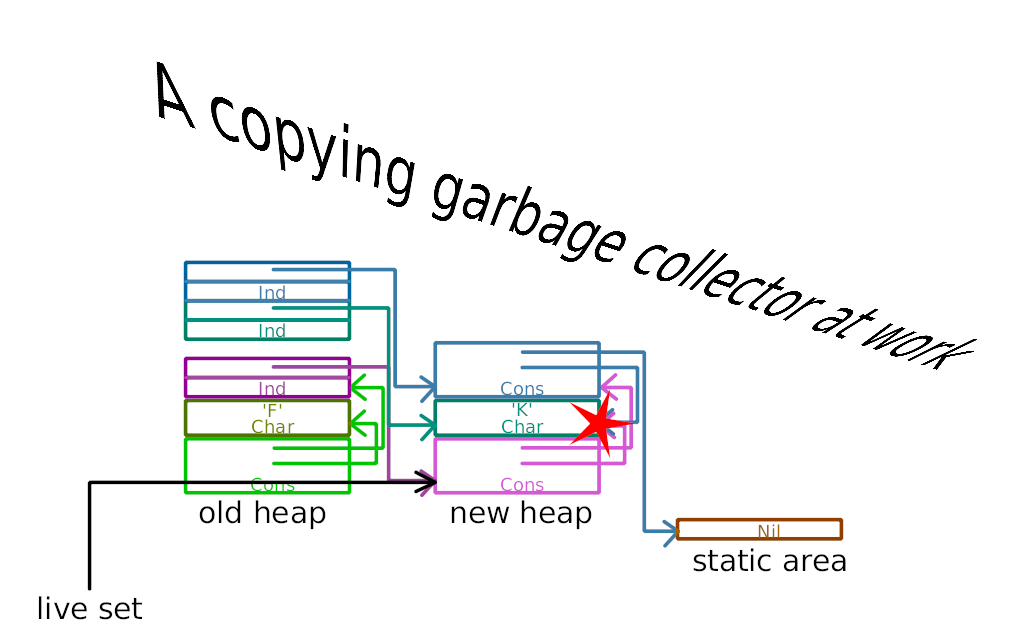
\includegraphics[width=.6\linewidth]{GC.png}
\end{center}

Es gibt noch einen weiteren Effekt den man hier jetzt gesehen hätte, würden wir das Programm wirklich ausführen (und nicht im Interpreter laufen lassen). Dann wäre die Ausgabe nämlich:
\begin{shell}
$ ./HelloGC 
0x00007f16c0d04270/2: 0x000000000049B1C8 0x00007F16C0D04261 0x00007F16C0D04240
0x00007f16c0d04260/1: 0x000000000049B128 0x0000000000000068
0x00007f16c0d162b0/2: 0x000000000049B1C8 0x00007F16C0D162A1 0x00007F16C0D16280
0x00007f16c0d162a0/1: 0x000000000049B128 0x0000000000000061
0x00007f16c0d262b0/2: 0x000000000049B1C8 0x00007F16C0D262A1 0x00007F16C0D26280
0x00007f16c0d262a0/1: 0x000000000049B128 0x000000000000006C
0x00007f16c0d362b0/2: 0x000000000049B1C8 0x00007F16C0D362A1 0x00007F16C0D36280
0x00007f16c0d362a0/1: 0x000000000049B128 0x000000000000006C
0x00007f16c0d462b0/2: 0x000000000049B1C8 0x00007F16C0D462A1 0x00007F16C0D46280
0x00007f16c0d462a0/1: 0x000000000049B128 0x000000000000006F
0x00000000006fb188/1: 0x000000000049B1A8
0x00007f16c0dfd4b8/2: 0x000000000049B1C8 0x00000000006FBAD1 0x00007F16C0DFD51A
0x00000000006fbad0/1: 0x000000000049B148 0x0000000000000068
0x00007f16c0dfd518/2: 0x000000000049B1C8 0x00000000006FBA61 0x00007F16C0DFD552
0x00000000006fba60/1: 0x000000000049B148 0x0000000000000061
0x00007f16c0dfd550/2: 0x000000000049B1C8 0x00000000006FBB11 0x00007F16C0DFD56A
0x00000000006fbb10/1: 0x000000000049B148 0x000000000000006C
0x00007f16c0dfd568/2: 0x000000000049B1C8 0x00000000006FBB11 0x00007F16C0DFD582
0x00000000006fbb10/1: 0x000000000049B148 0x000000000000006C
0x00007f16c0dfd580/2: 0x000000000049B1C8 0x00000000006FBB41 0x00000000006FB189
0x00000000006fbb40/1: 0x000000000049B148 0x000000000000006F
0x00000000006fb188/1: 0x000000000049B1A8
\end{shell}
und wir sehen dass nach dem Garbage Collector die Closures für das \li-'l'- identisch sind (beide zeigen nun auf \li-0x00000000006FBB11-) und im statischen Codebereich liegen. Das ist eine Optimierung speziell für \li-Char-s im ASCII-Bereich und für \li-Int-s mit Betrag bis zu 16. 

Nun müssten wir den Speicherverbrauch von \li-string- abschätzen können. Wir haben 100000000 Bytes, die jeweils in einem \li-Char- abgespeichert werden. Da die aber alle aus dem ASCII-Bereich sind, kosten sie nichts. Die Liste selbst jedoch braucht für jede Zelle drei Wörter á 8 Bytes, das sind fast die beobachteten 2521MB Speicherverbrauch. (Warum nicht das Dopplete? Weil der Garbage Collector nicht immer den gesamten Speicher kopiert sondern ihn in Generationen aufteilt – was wir hier nicht weiter vertiefen wollen.)

An dieser Stelle sollte klar sein dass sich der eingebaute \li-String--Datentyp \emph{nicht} für schnellen und speichereffizienten Code eignet. Es gibt Alternativen, allen voran \li-ByteString- für rohe Bytes und \li-Text- für Unicode-Text.

\subsection{Funktionen}

Wenden wir uns nun der nächsten Art von Closures zu, nämlich Funktionen. Weil es hier interpretiert recht anders als kompiliert funktioniert lasse ich folgendes Programm laufen:

\inputhaskell{FunClosures.hs}
was zu folgender Ausgabe führt:
\begin{shell}
$ ghc --make FunClosures.hs -O && ./FunClosures  1 2 3
0x00000000006f3090/2: 0x0000000000420DD8
0x00000000006ef7f0/1: 0x0000000000406408
0x00007f73f8d0e880/2
0x00007f73f8d10348/1: 0x0000000000406498 0x00007F73F8D0E882
\end{shell}
Einfache Funktionen liegen im statischen Code-Bereich und enhalten genau einen Pointer irgendwo hin. Das gilt auch für lokal definierte Funktionen. Interessant ist die Funktion \li-h-. Diese verwendet einen Wert (\li-a-) aus einer lokalen Variable. Das heißt der Code für \li-main- legt eine neue Funktionen-Closure auf dem Heap an, die zwei Wörter groß ist: Ein Verweis auf den statischen Code und eine Referenz auf den Wert von \li-a-. 

\subsection{Thunks}

Das wars erstmal von den Funktionen und wir wenden uns Thunks zu, die in gewisser weise nichts anderes sind als Funktionen ohne Parameter. Da es jetzt langsam kompliziert wird schauen wir uns nicht mehr den Speicher direkt an, sondern verwenden \li!ghc-vis!, ein Tool das Dennis Felsing in seiner Bachelorarbeit bei mir gerade entwickelt. Wir probieren folgenden Code im Modul \li-InfLists-
\begin{haskell}
infList f x = f x : infList f x
l = infList (+19) 23
\end{haskell}
mittels
\begin{ghci}
Prelude Inflists> :script /home/jojo/dokumente/Uni/WM/arbeiten/lazy-vis/vis/ghci
Prelude Inflists> :vis
Prelude Inflists> :switch
Prelude Inflists> :view l
\end{ghci}
und klicken auf dem entstehenden Baum herum. Wichtige Beobachtungen:
\begin{itemize}
\item Die Liste scheint sich tatsächlich unendlich unendlich abzurollen.
\item Der Wert 42 wird jedes mal neu berechnet und neu gespeichert.
\end{itemize}

Schön ist es jetzt auch noch
\begin{haskell}
l2 = map negate l
\end{haskell}
anzuschauen und zu beobachten, wie die Auswertung der einen Liste die andere beeinflusst.

\begin{center}
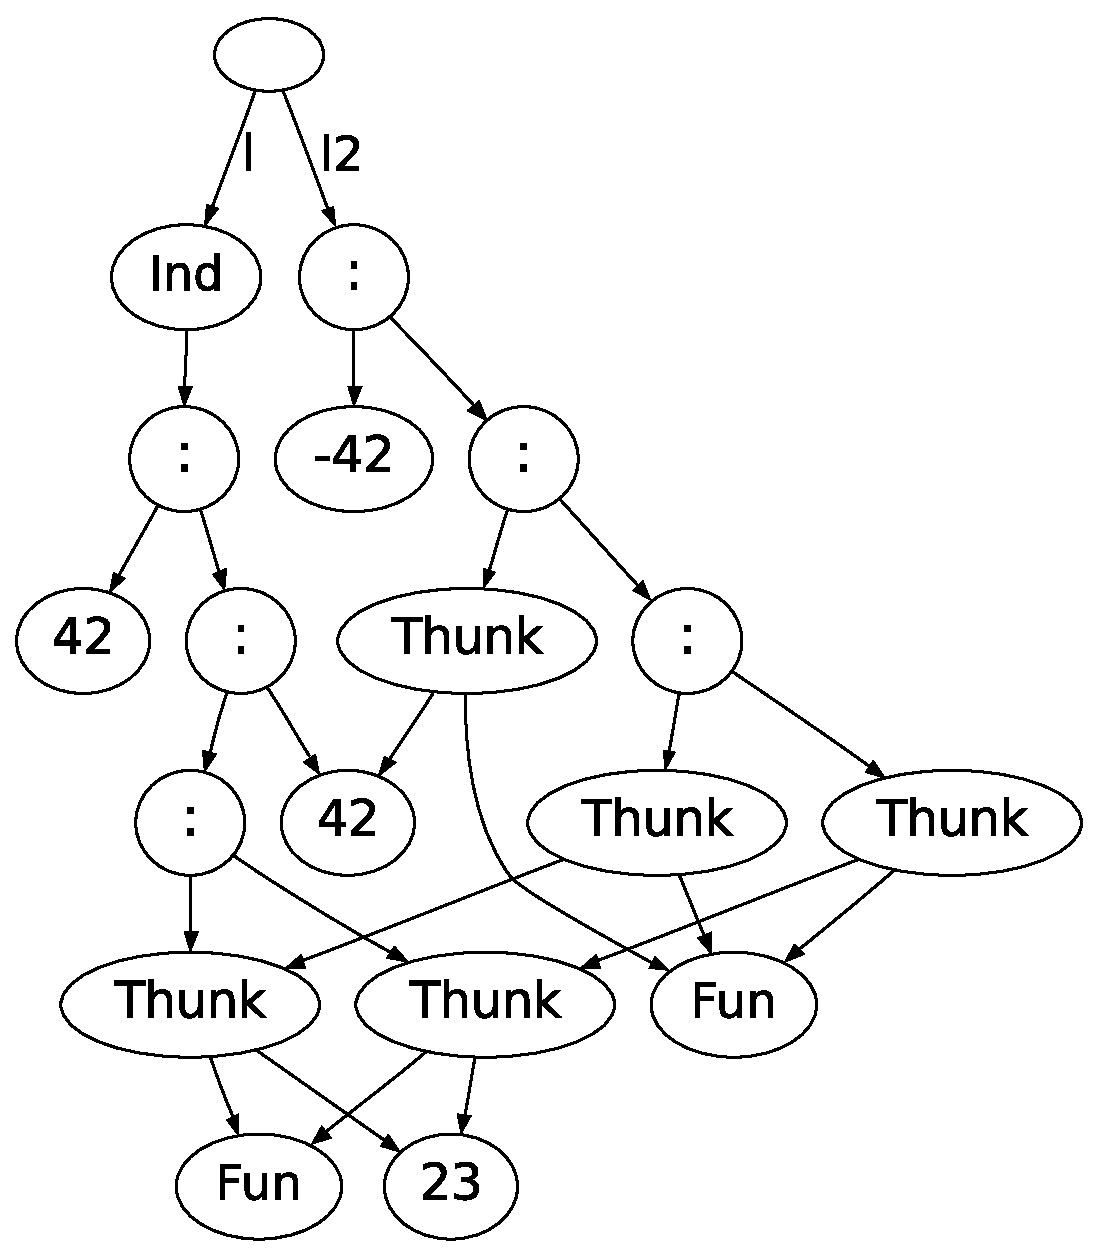
\includegraphics[width=0.4\linewidth]{vis-output1.pdf}
\end{center}

Zum Vergleich nehmen wir diese Funktion für unendliche Listen, die -- semantisch -- das gleiche macht:
\begin{haskell}
infList2 f x = let l = f x : l in l
\end{haskell}
und untersuchen \li-l3 = infList2 (+19) (23::Int)- mit \li-:view-. Tatsächlich wird hier die Cons-Zelle und die 42 nur jeweils einmal berechnet, danach zeigt der Tail der Liste wieder auf die Liste selbst. Auf diese Weise schafft es Haskell tatsächlich, eine unendliche Listen in endlich viel Speicher zu speichern!

Leider sind solche selbstbezüglichen Datenstrukturen fragil, wenn man sie „ändern“ will; schon ein einfaches \li-map negate l2- zerstört die Struktur, wie man hier gut sehen kann.

\begin{center}
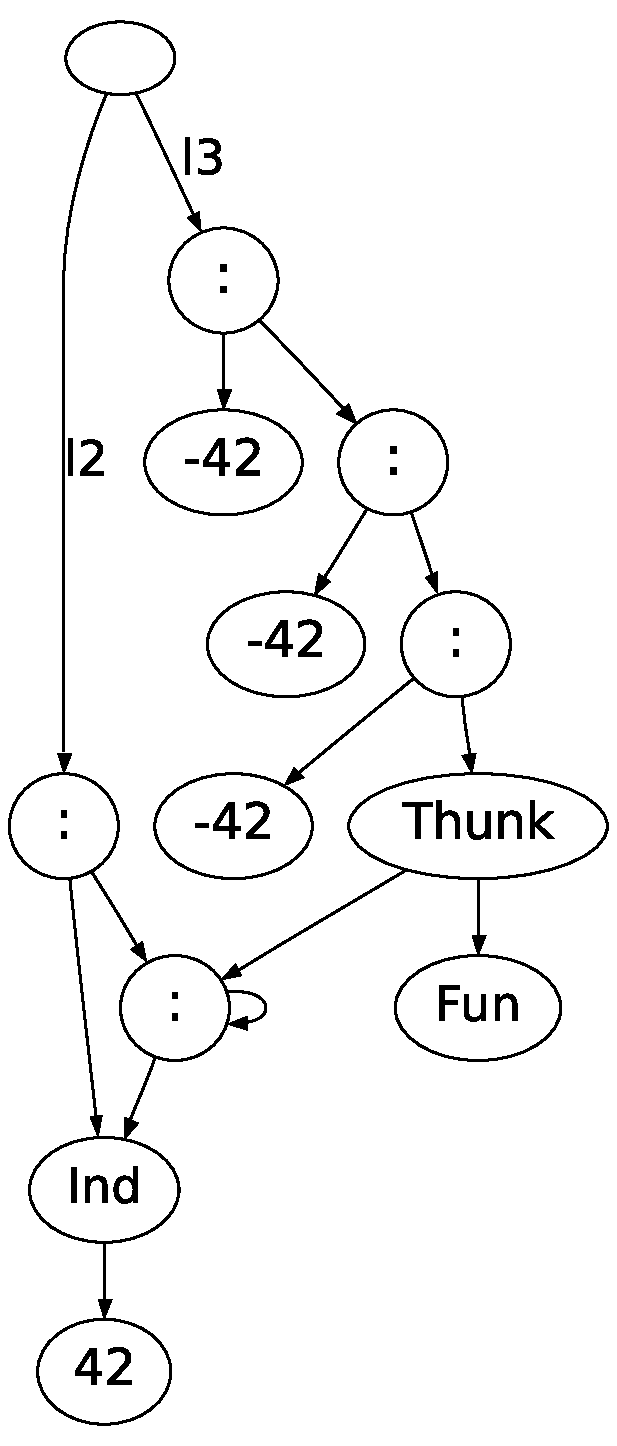
\includegraphics[width=0.2\linewidth]{vis-output2.pdf}
\end{center}

An dieser Stelle will ich wieder auf das zweite Beispiel vom Anfang zurückkommen. Jetzt können wir mit \li!ghc-vis! dem Stack Overflow auf den Grund gehen: 
\begin{ghci}
*Count> :switch
*Count> let x = count 0 [1..5]
*Count> :view x
\end{ghci}
Wir sehen ganze viele Thunks, die nacheinander die \li-0- modifizieren. Das sind eben die Thunks, die für \li-(+1)- stehen. Macht ja auch Sinn: Bevor wir die Zahl nicht benötigen, wird keine Berechnung ausgeführt. Trotzdem muss die Berechnung ja gespeichert werden. Klickt man auf einen der Thunks, kollabiert der Turm darunter in einem Rutsch.

Besser ist folgender Code:
\lstinputlisting[style=haskell,linerange=8-10]{Count.hs}\mylabel{Haskell}
Der Operator \li-$!$- sorgt dafür, dass das Argument (hier \li-n+1-) ausgewertet wird, bevor die Funktion (hier \li-count2-) aufgerufen wird. Dadurch wird stets nur eine Zahl, und kein Thunk, übergeben. Es tritt kein Stack Overflow auf, der Speicherverbrauch ist Konstant (und mit \li!ghc-vis! gibt es nichts zu sehen):
\begin{ghci}
*Count> let x = count2 0 [1..100000000]
*Count> x
100000000
\end{ghci}
Nur der Ehrlichkeit halber: Bei diesem einfachen Programm hätte der Compiler das auch selbst gemacht, wenn ich die Funktion nicht durch das \li-Just- künstlich nicht-strikt im Argument gemacht hätte.


\section{Der Info-Pointer}

Zum Schluss will ich noch darauf eingehen, was das erste Wort jedes Closures ist. Ihr habt vielleicht schon beobachtet, dass es stets in den statischen Code-Bereich zeigt. Und euch ist sicher schon aufgefallen, dass die Information, welcher Konstruktor das denn gerade ist, oder wo der ausführbare Code einer Funktion steht, ja noch irgendwo stehen muss. All das, und noch viel mehr, versteckt sich hinter dem Info-Pointer:

\def\ux{2.8cm}\def\uy{0.6cm}
\begin{center}
\begin{tikzpicture}[x=\ux, y=\uy,
	word/.style={shape=rectangle, draw, minimum width=\ux, minimum height=\uy}
	,halfword/.style={shape=rectangle, draw, minimum width=0.5*\ux, minimum height=\uy}
	,>=latex]
\draw (0,0) rectangle +(1,1) node[midway] (ip) {Info-Pointer}
    ++(1,0) rectangle +(1,1) node[midway] {Pointer}
    ++(1,0) rectangle +(1,1) node[midway] {Pointer}
    ++(1,0) +(0.1,0.4) node {$\cdots$}
    ++(0.2,0) rectangle +(1,1) node[midway] {Nicht-Pointer}
    ++(1,0) rectangle +(1,1) node[midway] {Nicht-Pointer}
    ++(1,0) +(0.1,0.4) node {$\cdots$};

\begin{scope}[yshift=-0.7cm, xshift=1.2*\ux]
\draw
  (0,0) node[word] (tbl) {Code-Pointer}
++(-0.25,-1) node[halfword] {\#ptr} ++(+0.5,0) node[halfword] {\#nptr} ++(-0.25,0)
++(-0.25,-1) node[halfword] {Typ} ++(+0.5,0) node[halfword] {SRT} ++ (-0.25,0)
++(0,-1) node[word] {ggf. Konstruktor}
++(0,-1) node[word] {ggf. Stelligkeit};
\end{scope}
\draw[*->] (ip.south) |- (tbl.west);
\draw[*->] (tbl.east) -- ++(1.5cm,0) node[right] (code) {Entry code};
\draw (code) ++(-0.5,-1) -- ++(0,1.5) -- ++(1,0) -- ++(0,-1.5);
\end{tikzpicture}
\end{center}

Hier ist noch interessant dass die Parameter eines Konsturktors bzw. die freien Variablen einer Funktion stets so angeordnet sind, dass erst die Zeiger und dann die anderen Werte kommen. Damit kann die Größe und das Layout des Closures in zwei Halbworten gespeichert werden, die sich der Garbage Collector anschaut, ohne eigenen Code für jeden Konstruktor zu benötigen.

Was aber am häufigsten mit so einem Closure passiert ist, dass er ausgeführt wird. Daher sieht das ganze in Wirklichkeit nochmal anders aus. Der Zeiger im Closure zeigt direkt an den Anfang des Funktionscodes, und der Compiler legt die Tabelle direkt davor. Das ist zwar eine unübliche Mischung von Daten und Code, aber der Compiler darf sowas.

\begin{center}
\begin{tikzpicture}[x=\ux, y=\uy,
	word/.style={shape=rectangle, draw, minimum width=\ux, minimum height=\uy}
	,halfword/.style={shape=rectangle, draw, minimum width=0.5*\ux, minimum height=\uy}
	,>=latex]
\draw (0,0) rectangle +(1,1) node[midway] (ip) {Info-Pointer}
    ++(1,0) rectangle +(1,1) node[midway] {Pointer}
    ++(1,0) rectangle +(1,1) node[midway] {Pointer}
    ++(1,0) +(0.1,0.4) node {$\cdots$}
    ++(0.2,0) rectangle +(1,1) node[midway] {Nicht-Pointer}
    ++(1,0) rectangle +(1,1) node[midway] {Nicht-Pointer}
    ++(1,0) +(0.1,0.4) node {$\cdots$};

\begin{scope}[yshift=-0.7cm, xshift=1.2*\ux]
\draw
  (0,0) node[word] {ggf. Konstruktor}
++(0,-1) node[word] {ggf. Stelligkeit}
++(-0.25,-1) node[halfword] {\#ptr} ++(+0.5,0) node[halfword] {\#nptr} ++(-0.25,0)
++(-0.25,-1) node[halfword] {Typ} ++(+0.5,0) node[halfword] {SRT} ++ (-0.25,0)
++(0,-1) node[word,draw=none] (code) {Entry code};
\end{scope}
\draw[*->] (ip.south) |- (code.west);
\draw (code) ++(-0.5,-1) -- ++(0,1.5) -- ++(1,0) -- ++(0,-1.5);
\end{tikzpicture}
\end{center}


\section{Das Primzahlensieb}

Falls es die Zeit erlaubt will ich noch einem weiteren Programm bei der Ausführung zuschauen, nämlich der bekannten, sehr eleganten Definition der Primzahlen:
\inputhaskell{Sieve.hs}
Hier erkennt man schön die immer länger werdende Liste von Thunks, die jeweils für eine Primzahl deren vielfache aus der Liste entfernt:

\begin{center}
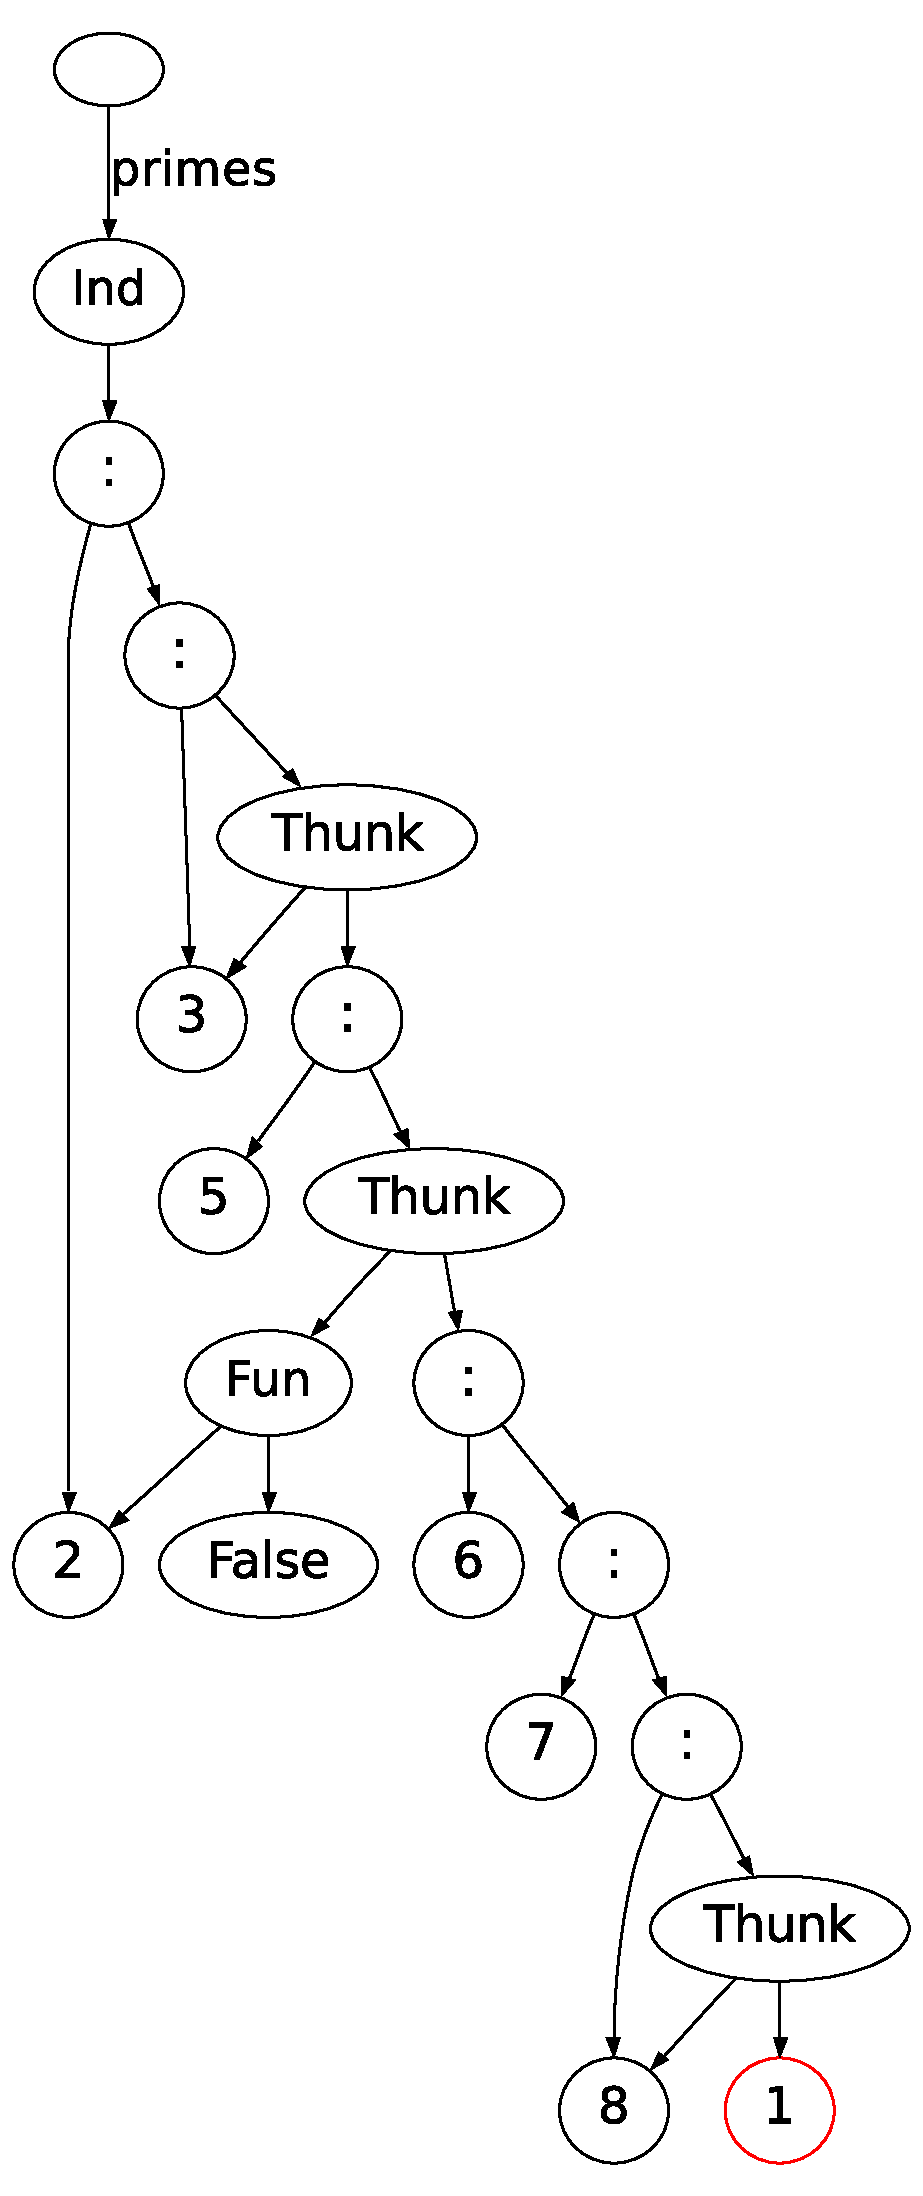
\includegraphics[width=0.2\linewidth]{vis-output-sieve.pdf}
\end{center}

\section{Fazit}

Damit bin ich am Ende meines Vortrages. Wir haben uns die Mühe gemacht, all die vielen komfortablen Abstraktionsschichten, die uns Haskell bereitstellt, beiseite zu schieben und haben einen ungetrübten Blick auf den Speicher geworfen. Wir haben gesehen dass die Daten doch einigermaßen übersichtlich und effizient gespeichert werden. Wir haben auch gesehen, warum \li-Strings-s so teuer sind und wie man eine unendlich lange Liste in wenigen Bytes speichert. Ich hoffe, dass euch dieser Vortrag hilft besser zu verstehen, warum eure Haskell-Programme so laufen wie sie laufen, und zu wissen, wie ihr sie besser laufen lassen könnt.

\section{Referenzen}

\begin{itemize}
\item Was wir hier gesehen haben ist in der Wissenschaft als \emph{Spineless, tagless G-machine} bekannt. \url{http://citeseerx.ist.psu.edu/viewdoc/summary?doi=10.1.1.53.3729}
\item Das GHC-Wiki beschreibt die aktuelle Implementierung am pragmatischten, insbesondere \url{http://hackage.haskell.org/trac/ghc/wiki/Commentary/Rts/Storage/HeapObjects}.
\item Wir haben hier meine Bibliothek ghc-heap-view (\url{http://hackage.haskell.org/package/ghc-heap-view}) und Dennis Felsing’s \li!ghc-vis! (\url{http://felsin9.de/nnis/ghc-vis/}) verwendet.
\item Das Video habe ich mit Synfig erstellt. (\url{http://www.synfig.org/})
\end{itemize}


\end{document}

